\documentclass[../main.tex]{subfiles}
 
\begin{document}

% overview
% visual depiction of results
% performance described in text that references the visuals
% performance discussed in text – did it work well? why or why not?

This section presents the classification results for the two model types on the two datasets. Results indicate that both the \acl{mlp} and the \acl{cnn} can adequately classify \ac{can} data segments, but the \ac{cnn} is certainly better than the \ac{mlp} on both the imbalanced dataset and the balanced dataset. Results also indicate that both models perform better on the larger, imbalanced dataset; this is simply due to the availability of training data in each set. Table \ref{tab:balanced-accuracy} presents the overall balanced accuracies.

\begin{table}
    \caption{Balanced Accuracy for Each Model}
    \centering
    \label{tab:balanced-accuracy}
    \begin{tabular}{|c|c|c|}
    \hline
    \textbf{Model} & \textbf{Dataset} & \textbf{Accuracy} \\
    \hline
    Multi-layer perceptron       & Imbalanced & 81.71 \% \\
    Multi-layer perceptron       & Balanced   & 76.95 \% \\
    Convolutional neural network & Imbalanced & 83.18 \% \\
    Convolutional neural network & Balanced   & 80.94 \% \\
    \hline
    \end{tabular}
\end{table}

Table \ref{tab:all-accuracy} presents class-specific accuracy values for the four trained models. The grey cells indicate the best model/dataset combination for each of the 20 vehicles. Clearly, the \ac{cnn} trained on the imbalanced dataset performs better than the other trained models on a majority (13/20) of the classes, and it does not give the worst overall performance for any of the classes. This is further evidence of the superior performance of the \ac{cnn}, and it also indicates that more training data is better, even if the classes in said data are (severely) imbalanced.

\begin{table}
    \caption{Class Accuracy for Each Vehicle}
    \centering
    \label{tab:all-accuracy}
    \begin{tabular}{|c|c|c|c|c|c|}
    \hline
    \textbf{Vehicle} & \textbf{MLP Imbalanced} & \textbf{MLP Balanced} & \textbf{CNN Imbalanced} & \textbf{CNN Balanced} & \textbf{Median} \\
    \hline
    1 & \cellcolor{grey}98.31 \% & 83.29 \% & 92.58 \% & 88.20 \% & 90.39 \\
    2 & 86.89 \% & 76.61 \% & \cellcolor{grey}88.69 \% & 80.88 \% & 83.88 \\
    3 & 93.59 \% & 81.82 \% & \cellcolor{grey}93.60 \% & 74.21 \% & 87.70 \\
    4 & 94.40 \% & 76.52 \% & \cellcolor{grey}94.55 \% & 77.87 \% & 86.13 \\
    5 & 96.85 \% & 70.72 \% & \cellcolor{grey}97.56 \% & 81.57 \% & 89.21 \\
    6 & \cellcolor{grey}96.20 \% & 94.72 \% & 94.72 \% & 83.63 \% & 94.72 \\
    7 & 89.50 \% & 70.47 \% & \cellcolor{grey}92.71 \% & 48.27 \% & 79.98 \\
    8 & 94.99 \% & 92.49 \% & \cellcolor{grey}96.85 \% & 89.34 \% & 93.74 \\
    9 & 96.03 \% & 86.26 \% & \cellcolor{grey}98.34 \% & 92.64 \% & 94.33 \\
    101 & 87.54 \% & 60.22 \% & \cellcolor{grey}89.00 \% & 83.38 \% & 85.46 \\
    102 & \cellcolor{grey}97.63 \% & 84.31 \% & 82.51 \% & 75.56 \% & 83.41 \\
    103 & 85.67 \% & 89.51 \% & \cellcolor{grey}93.57 \% & 81.59 \% & 87.59 \\
    104 & 83.18 \% & \cellcolor{grey}89.55 \% & 89.29 \% & 87.83 \% & 88.56 \\
    105 & 91.80 \% & 50.83 \% & 93.94 \% & \cellcolor{grey}94.83 \% & 92.87 \\
    106 & 89.38 \% & \cellcolor{grey}89.70 \% & 85.59 \% & 85.17 \% & 87.48 \\
    107 & 82.52 \% & 69.44 \% & \cellcolor{grey}87.41 \% & 79.26 \% & 80.89 \\
    108 & 94.42 \% & 73.61 \% & \cellcolor{grey}95.12 \% & 89.64 \% & 92.03 \\
    109 & 90.79 \% & 85.71 \% & \cellcolor{grey}93.60 \% & 82.67 \% & 88.25 \\
    110 & 82.18 \% & 84.50 \% & 83.78 \% & \cellcolor{grey}87.81 \% & 84.14 \\
    111 & 74.01 \% & 70.98 \% & \cellcolor{grey}88.07 \% & 78.80 \% & 76.40 \\
    \hline
    \end{tabular}
\end{table}

% transition paragraph

Figure \ref{fig:matrix} presents the multiclass confusion matrices for both model types and both datasets. Generally, one can see that each model tends to correctly classify \ac{can} segments, but some specific misclassifications are certainly common. For example, all four models misclassify Vehicle 106 as Vehicle 107 (and vice versa) to some extent; these are different-year Honda Accords. Similarly, the models often confuse Vehicles 2 and 111, the two 2009 Toyota Corollas in the dataset. One can also see that the models often perform well on the same vehicle. For example, all models demonstrate strong performance on Vehicle 8---perhaps Subaru employed a distinct \ac{can} format when designing its 2017 WRX. One can easily discern other trends by further analyzing Figure \ref{fig:matrix}.

\begin{figure}
    \centerline{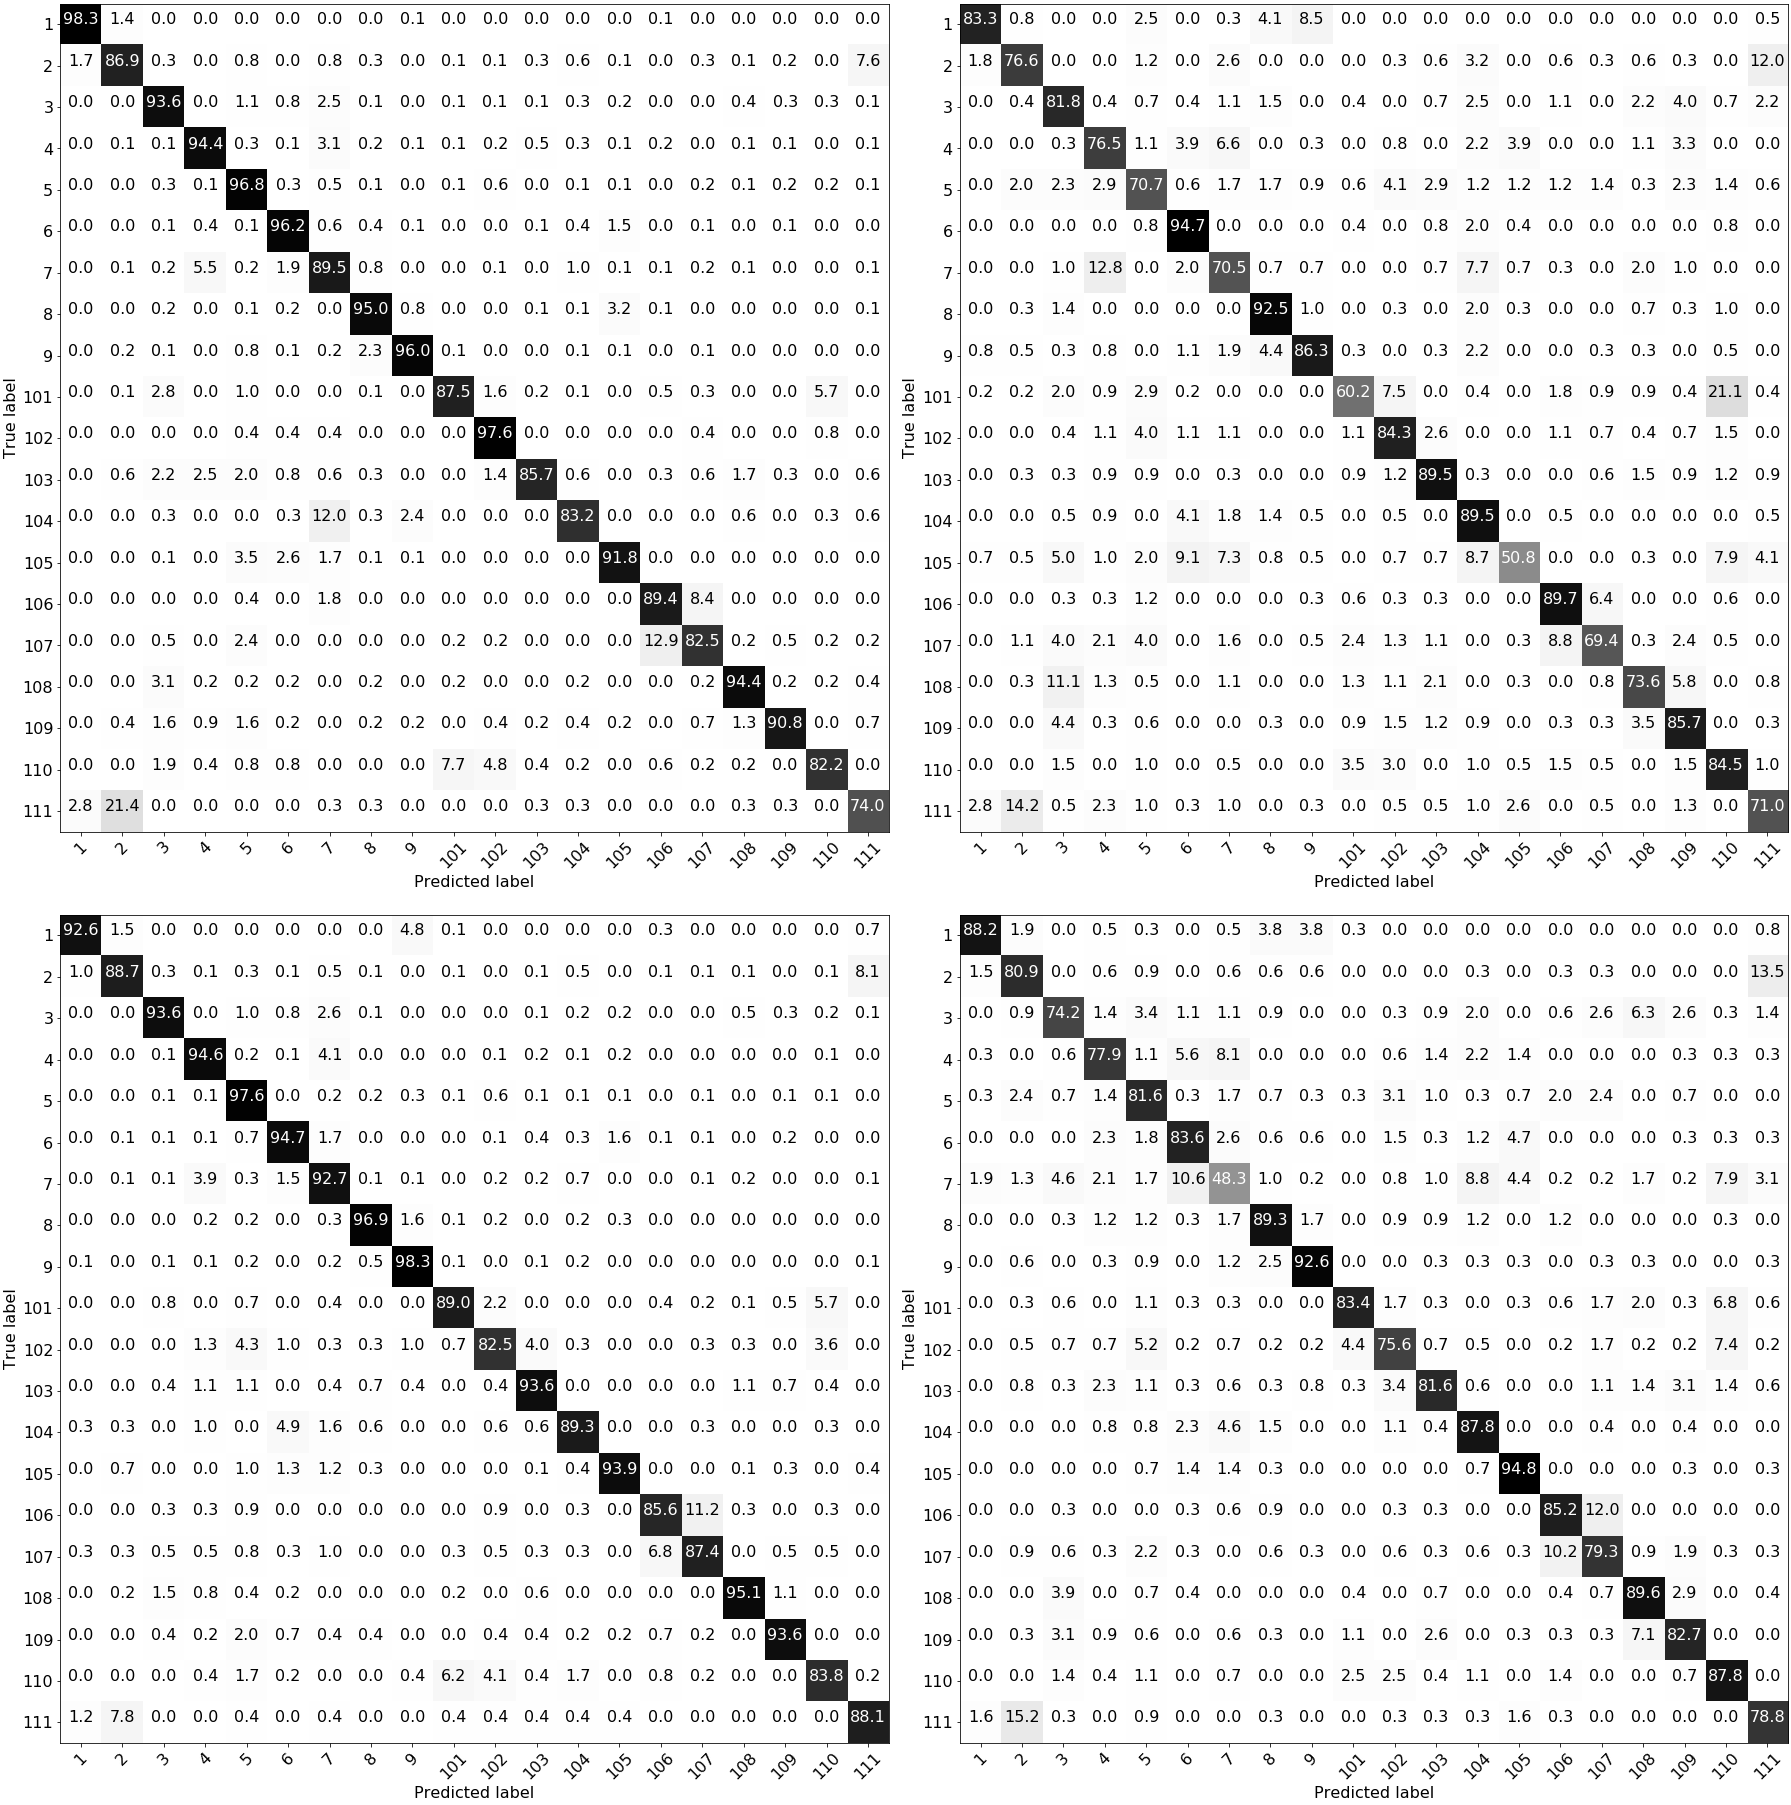
\includegraphics[scale=0.2875]{matrix.png}}
    \caption{Confusion matrices. \textit{Top left:} \acl{mlp} on the imbalanced dataset; \textit{Top right:} \acl{mlp} on the balanced dataset; \textit{Bottom left:} \acl{cnn} on the imbalanced dataset; \textit{Bottom right:} \acl{cnn} on the balanced dataset.}
    \label{fig:matrix}
\end{figure}

Section \ref{sec:conclusion} discusses the real-world implications of these results. Additionally, the section offers areas for future research in \ac{can} analysis and security.

\end{document}
